%% BioMed_Central_Tex_Template_v1.06
%%                                      %
%  bmc_article.tex            ver: 1.06 %
%                                       %

%%IMPORTANT: do not delete the first line of this template
%%It must be present to enable the BMC Submission system to
%%recognise this template!!

%%%%%%%%%%%%%%%%%%%%%%%%%%%%%%%%%%%%%%%%%
%%                                     %%
%%  LaTeX template for BioMed Central  %%
%%     journal article submissions     %%
%%                                     %%
%%          <8 June 2012>              %%
%%                                     %%
%%                                     %%
%%%%%%%%%%%%%%%%%%%%%%%%%%%%%%%%%%%%%%%%%


%%%%%%%%%%%%%%%%%%%%%%%%%%%%%%%%%%%%%%%%%%%%%%%%%%%%%%%%%%%%%%%%%%%%%
%%                                                                 %%
%% For instructions on how to fill out this Tex template           %%
%% document please refer to Readme.html and the instructions for   %%
%% authors page on the biomed central website                      %%
%% http://www.biomedcentral.com/info/authors/                      %%
%%                                                                 %%
%% Please do not use \input{...} to include other tex files.       %%
%% Submit your LaTeX manuscript as one .tex document.              %%
%%                                                                 %%
%% All additional figures and files should be attached             %%
%% separately and not embedded in the \TeX\ document itself.       %%
%%                                                                 %%
%% BioMed Central currently use the MikTex distribution of         %%
%% TeX for Windows) of TeX and LaTeX.  This is available from      %%
%% http://www.miktex.org                                           %%
%%                                                                 %%
%%%%%%%%%%%%%%%%%%%%%%%%%%%%%%%%%%%%%%%%%%%%%%%%%%%%%%%%%%%%%%%%%%%%%

%%% additional documentclass options:
%  [doublespacing]
%  [linenumbers]   - put the line numbers on margins

%%% loading packages, author definitions

\documentclass[twocolumn]{bmcart}% uncomment this for twocolumn layout and comment line below
%\documentclass{bmcart}

%%% Load packages
%\usepackage{amsthm,amsmath}
%\RequirePackage{natbib}
%\RequirePackage[authoryear]{natbib}% uncomment this for author-year bibliography
%\RequirePackage{hyperref}
\usepackage[utf8]{inputenc} %unicode support
\usepackage[english]{babel}
\usepackage{graphicx}
%\usepackage[applemac]{inputenc} %applemac support if unicode package fails
%\usepackage[latin1]{inputenc} %UNIX support if unicode package fails


%%%%%%%%%%%%%%%%%%%%%%%%%%%%%%%%%%%%%%%%%%%%%%%%%
%%                                             %%
%%  If you wish to display your graphics for   %%
%%  your own use using includegraphic or       %%
%%  includegraphics, then comment out the      %%
%%  following two lines of code.               %%
%%  NB: These line *must* be included when     %%
%%  submitting to BMC.                         %%
%%  All figure files must be submitted as      %%
%%  separate graphics through the BMC          %%
%%  submission process, not included in the    %%
%%  submitted article.                         %%
%%                                             %%
%%%%%%%%%%%%%%%%%%%%%%%%%%%%%%%%%%%%%%%%%%%%%%%%%


%\def\includegraphic{}
%\def\includegraphics{}



%%% Put your definitions there:
\startlocaldefs
\endlocaldefs


%%% Begin ...
\begin{document}

%%% Start of article front matter
\begin{frontmatter}

\begin{fmbox}
\dochead{Report}

%%%%%%%%%%%%%%%%%%%%%%%%%%%%%%%%%%%%%%%%%%%%%%
%%                                          %%
%% Enter the title of your article here     %%
%%                                          %%
%%%%%%%%%%%%%%%%%%%%%%%%%%%%%%%%%%%%%%%%%%%%%%

\title{Alignment-free tools for metagenomics-data analysis}

%%%%%%%%%%%%%%%%%%%%%%%%%%%%%%%%%%%%%%%%%%%%%%
%%                                          %%
%% Enter the authors here                   %%
%%                                          %%
%% Specify information, if available,       %%
%% in the form:                             %%
%%   <key>={<id1>,<id2>}                    %%
%%   <key>=                                 %%
%% Comment or delete the keys which are     %%
%% not used. Repeat \author command as much %%
%% as required.                             %%
%%                                          %%
%%%%%%%%%%%%%%%%%%%%%%%%%%%%%%%%%%%%%%%%%%%%%%

\author[
   addressref={aff1},                   % id's of addresses, e.g. {aff1,aff2}
   corref={aff1},                       % id of corresponding address, if any
  % noteref={n1},                        % id's of article notes, if any
   email={robert.deibel@student.uni-tuebingen.de}   % email address
]{\inits{RD}\fnm{Robert} \snm{Deibel}}

%%%%%%%%%%%%%%%%%%%%%%%%%%%%%%%%%%%%%%%%%%%%%%
%%                                          %%
%% Enter the authors' addresses here        %%
%%                                          %%
%% Repeat \address commands as much as      %%
%% required.                                %%
%%                                          %%
%%%%%%%%%%%%%%%%%%%%%%%%%%%%%%%%%%%%%%%%%%%%%%

\address[id=aff1]{%                           % unique id
  \orgname{Eberhard-Karls Universität}, % university, etc
  %\street{Waterloo },                     %
  %\postcode{}                                % post or zip code
  \city{Tübingen},                              % city
  \cny{DE}                                    % country
}


%%%%%%%%%%%%%%%%%%%%%%%%%%%%%%%%%%%%%%%%%%%%%%
%%                                          %%
%% Enter short notes here                   %%
%%                                          %%
%% Short notes will be after addresses      %%
%% on first page.                           %%
%%                                          %%
%%%%%%%%%%%%%%%%%%%%%%%%%%%%%%%%%%%%%%%%%%%%%%

\begin{artnotes}
%\note{Sample of title note}     % note to the article
%\note[id=n1]{Equal contributor} % note, connected to author
\end{artnotes}

%\end{fmbox}% comment this for two column layout

%%%%%%%%%%%%%%%%%%%%%%%%%%%%%%%%%%%%%%%%%%%%%%
%%                                          %%
%% The Abstract begins here                 %%
%%                                          %%
%% Please refer to the Instructions for     %%
%% authors on http://www.biomedcentral.com  %%
%% and include the section headings         %%
%% accordingly for your article type.       %%
%%                                          %%
%%%%%%%%%%%%%%%%%%%%%%%%%%%%%%%%%%%%%%%%%%%%%%

\begin{abstractbox}

\begin{abstract} % abstract
	Metagenomics; as the study and analysis of microorganisms of biotopes, like the human gut, is a field of vast research where researchers have to deal with the giant sets of data gathered through NGS-methods. Since the amount of data results in stress on computation and time resources, the development of fast and light analysis tools is appreciated. In this report I want to introduce the two main branches of analysis tools, while setting the focus on alignment-free methods.\\
	While the alignment-based approach are based on alignments -- as seen with Smith-Waterman or BLAST -- alignment-free methods, which are the main part of this report, have different approaches. Here I will showcase a selection of statistical and machine learning approaches and test these methods on a selected metagenomic data set.\\ 
	 TODO
\end{abstract}

%%%%%%%%%%%%%%%%%%%%%%%%%%%%%%%%%%%%%%%%%%%%%%
%%                                          %%
%% The keywords begin here                  %%
%%                                          %%
%% Put each keyword in separate \kwd{}.     %%
%%                                          %%
%%%%%%%%%%%%%%%%%%%%%%%%%%%%%%%%%%%%%%%%%%%%%%

\begin{keyword}
\kwd{alignment-free}
\kwd{report}
\kwd{metagenome}
\end{keyword}

% MSC classifications codes, if any
%\begin{keyword}[class=AMS]
%\kwd[Primary ]{}
%\kwd{}
%\kwd[; secondary ]{}
%\end{keyword}

\end{abstractbox}
%
\end{fmbox}% uncomment this for twcolumn layout

\end{frontmatter}

%%%%%%%%%%%%%%%%%%%%%%%%%%%%%%%%%%%%%%%%%%%%%%
%%                                          %%
%% The Main Body begins here                %%
%%                                          %%
%% Please refer to the instructions for     %%
%% authors on:                              %%
%% http://www.biomedcentral.com/info/authors%%
%% and include the section headings         %%
%% accordingly for your article type.       %%
%%                                          %%
%% See the Results and Discussion section   %%
%% for details on how to create sub-sections%%
%%                                          %%
%% use \cite{...} to cite references        %%
%%  \cite{koon} and                         %%
%%  \cite{oreg,khar,zvai,xjon,schn,pond}    %%
%%  \nocite{smith,marg,hunn,advi,koha,mouse}%%
%%                                          %%
%%%%%%%%%%%%%%%%%%%%%%%%%%%%%%%%%%%%%%%%%%%%%%

%%%%%%%%%%%%%%%%%%%%%%%%% start of article main body
% <put your article body there>
\section*{Introduction}
\subsection*{Metagenomics}
\paragraph*{A puddle of mud}
The metagenome is the whole set of genes of a population of microorganisms as found in a sample of a microbiome, the DNA of organisms, expected to have differing taxonomy, is isolated form these samples. As such metagenomics is the study and analysis of these metagenomes.\cite{handelsman2004metagenomics}\\
A microbiome is the "home" of countless bacteria, archea and viruses; like all microorganisms $>$90\% of those found in microbioms are uncultured, leaving researchers with the problem of how to study those organisms.
%\paragraph*{Accumulated data from microbiome samples}

%Choosing a sample is the easiest part of the analysis of a microbiome; the following steps are:\\
%\begin{enumerate}
%	\item DNA isolation from samples
%	\item construction of DNA libraries (typically in \textit{E. Coli} as host)
%	\item Mining for clones and DNA sequences of interest
%	\item Accumulation of desired clones and DNA sequences
%\end{enumerate}
%as stated in Streit et al \cite{STREIT2004492}, to obtain a metagenomic library, which is the base of analysis.\\
\paragraph*{NGS -- Next Generation Sequencing}
The sheer amount of data gathered through such samples -- Kakirde et al\cite{KAKIRDE20101911} states 10000 Gb of DNA in a soil sample -- leaves researches with the problem of sequencing.\\
While Sanger sequencing is an accurate and proven method for sequencing it is dated for the scale of metagenomics. Nowadays new high throughput methods -- also Next Generation Sequencing or NGS for short -- are used to handle this problem. NGS is a conglomerate of methods used  for rapid parallelized sequencing, producing thousands or millions of sequences concurrently.\\
 After converting the data into sequences through NGS methods of bioinformatics can be applied to analyze these.
\paragraph*{What do we want to achieve?}
Researches use the information gained through metagenomic-data analysis to design antibiotics and medicine or to analyze the metabolism of microorganisms and its hosts. Due to the rising number of identified genes using metagenomics-data analysis (Figure \ref{img:nov_gene_discov}) and the  $>$90\% uncultured microorganisms, metagenomics is a field of vast research.\\
Following I want to briefly summarize two approaches to data analysis and showcase one of those in more detail.
\begin{figure}
	\centering
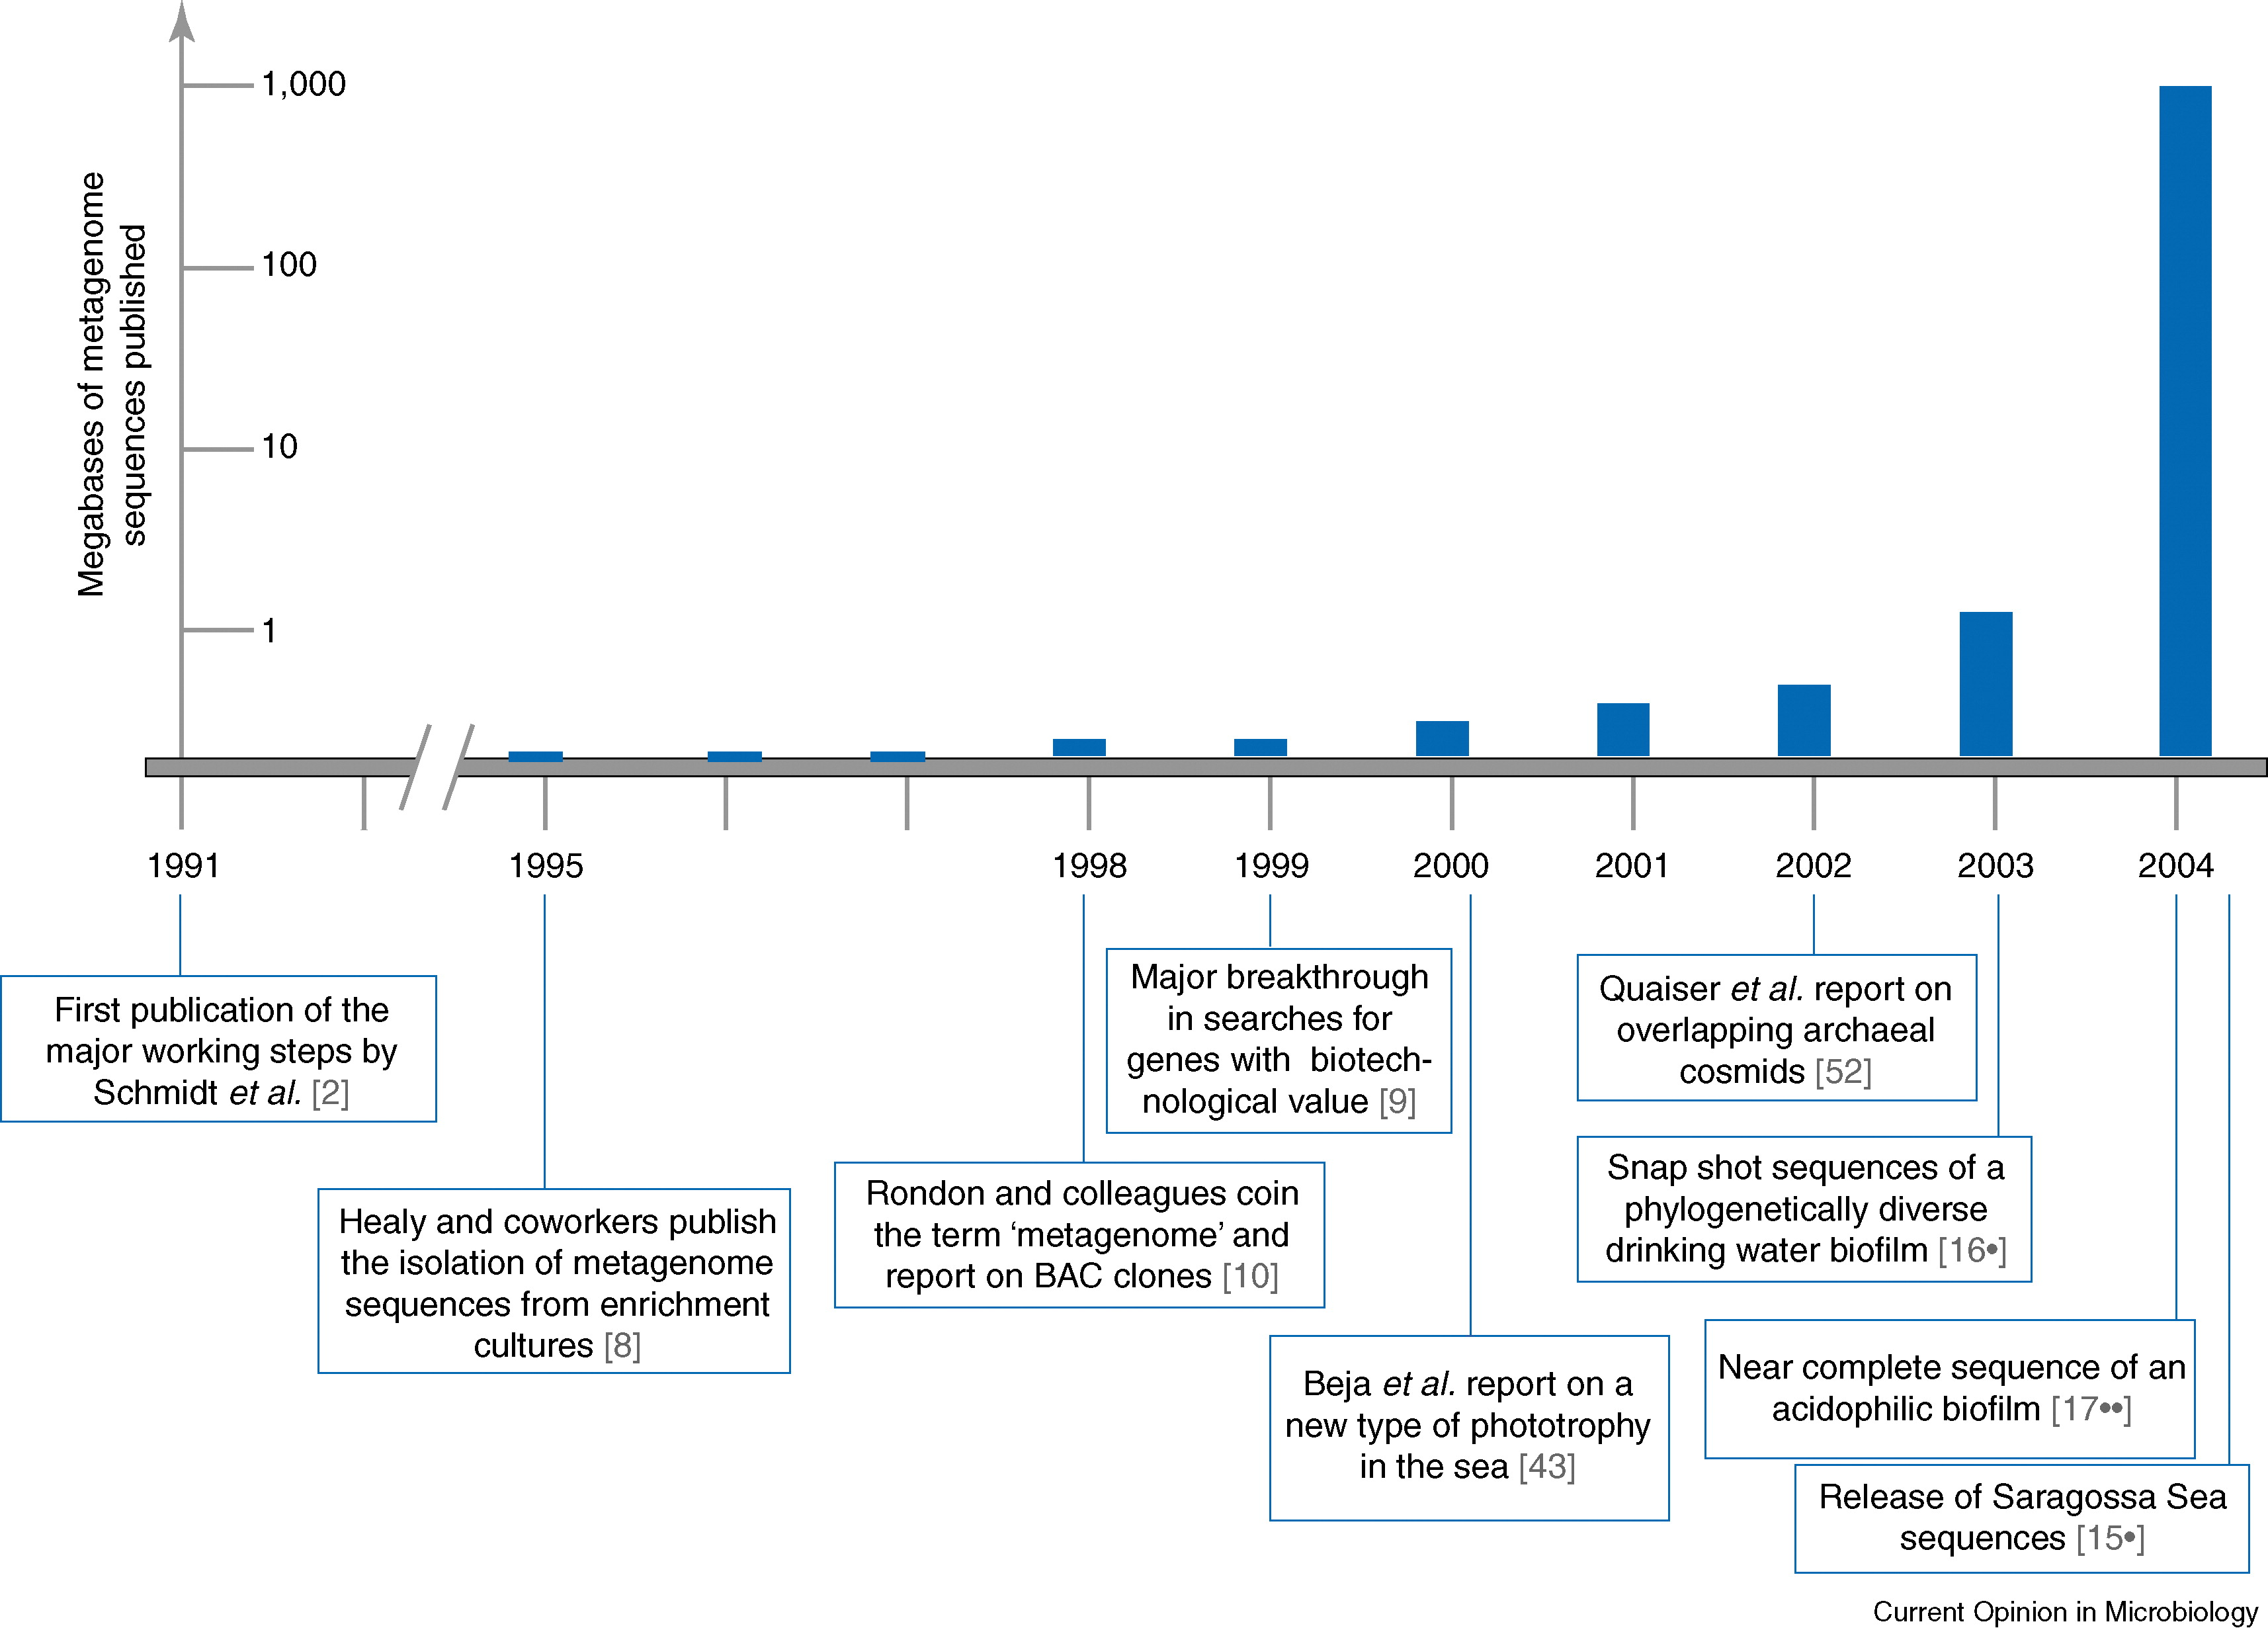
\includegraphics[width=.9\linewidth]{bilder/growth_of_novel_gene_discovery.jpg}	
\caption{Timescale of metagenomic-derived and published DNA sequences. The timescale ranges from 1991, the initial outline of the major working steps, to the first mapping of archaeal comids in 2002 and the snap shot sequence analysis of the Sargasso Sea published earlier this year.--taken from Streit et al \cite{STREIT2004492}}
\label{img:nov_gene_discov}
\end{figure}
\subsection*{The "classical" approach}
\paragraph*{Alignment-based method}
The best known approach to analyze sequences, metagenomic or not, is the alignment-based method. While this approach may vary depending on implementation and tool used it is the same underlying idea.\\
Gathered sequences are split into queries of substrings and aligned against a database of known and sequenced genomes while a scoring function is applied to weigh the  solution. These can then be analyzed and characterized depending on score, similarity, taxonomy and other factors.
\paragraph*{The good}
The here called classical approach is proven under various conditions and implemented numerous times. The accuracy of a BLAST-based analysis is well over 80\%\cite{doi:10.1142/9789814295291_0003}, while this seems as the perfect way to analyze our metagenomic-data -- even if BLAST is originally not designed for this purpose -- the drawbacks are visible under consideration of NGS.
\paragraph*{The bad -- Too much data, too little time}
NGS supplies researchers with a overabundance of novel data to be analyzed. This analysis of metagenomes is heavy on computation and time resources, due to the amount of data collected. BLAST aligns its queries with the entries in a chosen database -- for 10000Gb of data one can safely assume this step as time consuming -- this results in the pursuit of faster and more effective methods for data analysis. So the demand of lightweight tools with fast computation and unorthodox approaches is high and rising.
\subsection*{The alternative}
\paragraph*{Alignment-free method}
Apart from basing the analysis on alignment of sequences the other method would be to use alignment-free tools. While easily defined -- as a method of analyzing (metagenomic) data without the use of alignments -- the field itself is vast and filled with creative new approaches. For this report I reflect the work of Song et al \cite{doi:10.1093/bib/bbt067} and Laczny et al \cite{Laczny2014} both presenting methods for the analysis of metagenomic-data using alignment-free approaches. Basing their work on statistical methods and visualization respectively.
\section*{Methods}
\subsection*{Statistics}
\paragraph*{The power of statistics}

\subsection*{k-tupel approach -- Song et al}
\paragraph*{D$_2$}
\paragraph*{Nucleotide bias}
\subsection*{Visualization and machine learning}
\paragraph*{The idea behind}
Another method relies on the Barnes-Hut-SNE\cite{DBLP:journals/corr/abs-1301-3342} approach on machine learning, where high-dimensional data can be visualized in time $\mathcal{O}(n \log n)$ using vantage-point trees and a variant of the Barnes-Hut algorithm exceeding the speed of the prior used t-SNE approach ($\mathcal{O}(n^2)$).\\
Van der Maaten tried to optimize the t-SNE approach to machine learning through the idea that similar objects (in Euclidean space) have to be related to one another, thus different objects should be unrelated. On this assumption he based the BH SNE approach.
\paragraph*{probabilities and distance}
When using t-SNE, objects are described with points, a joint probability is assigned to the objects and a similarity function to the points. These can then be minimized using a Kullback-Leibler divergence. \cite{DBLP:journals/corr/abs-1301-3342} The computation of this algorithm is apparent as $\mathcal{O}(n^2)$, where $n$ is the number of objects. To lower this cost van der Maaten wanted to cut the computation of obvious not related objects, using a Barnes-Hut algorithm and metric trees.
\paragraph*{vantage-point trees and Barnes-Hut }
 The Barnes-Hut algorithm is often used by astronomers to perform $N$-body simulations.\cite{DBLP:journals/corr/abs-1301-3342} . In this algorithm it is assumed that the force of objects with sufficient distance to one another is infinitesimal and thus can be ignored in further computation. Leading --in the case of BH SNE -- to a cut in objects to include in calculations.\\
 For choosing these Objects van der Maaten used vantage-point trees, where similar nodes are saved as the left, dissimilar nodes as the right child. After establishing the data structure one can search the tree and apply the given algorithm to the nodes of interest resulting in a decrease of runtime.\\
 Originally this approach was intended for pattern recognition, but found a usage in bioinformatics.
\subsection*{BH SNE for metagenomics-- Laczny et al}
\paragraph*{Weiss noch nicht hier}
\section*{Results}
\subsection*{Application of tools on data set}
\paragraph*{hier kommt was hin}

%%%%%%%%%%%%%%%%
%% Background %%
%%
%\section*{Content}
%\section*{Section title}
%\subsection*{Sub-heading for section}
%\subsubsection*{Sub-sub heading for section}
%\paragraph*{Sub-sub-sub heading for section}

%%%%%%%%%%%%%%%%%%%%%%%%%%%%%%%%%%%%%%%%%%%%%%
%%                                          %%
%% Backmatter begins here                   %%
%%                                          %%
%%%%%%%%%%%%%%%%%%%%%%%%%%%%%%%%%%%%%%%%%%%%%%

\begin{backmatter}

\section*{Competing interests}

\section*{Author's contributions}

\section*{Acknowledgements}
%%%%%%%%%%%%%%%%%%%%%%%%%%%%%%%%%%%%%%%%%%%%%%%%%%%%%%%%%%%%%
%%                  The Bibliography                       %%
%%                                                         %%
%%  Bmc_mathpys.bst  will be used to                       %%
%%  create a .BBL file for submission.                     %%
%%  After submission of the .TEX file,                     %%
%%  you will be prompted to submit your .BBL file.         %%
%%                                                         %%
%%                                                         %%
%%  Note that the displayed Bibliography will not          %%
%%  necessarily be rendered by Latex exactly as specified  %%
%%  in the online Instructions for Authors.                %%
%%                                                         %%
%%%%%%%%%%%%%%%%%%%%%%%%%%%%%%%%%%%%%%%%%%%%%%%%%%%%%%%%%%%%%

% if your bibliography is in bibtex format, use those commands:
\bibliographystyle{bmc-mathphys} % Style BST file (bmc-mathphys, vancouver, spbasic).
\bibliography{bibliography}      % Bibliography file (usually '*.bib' )
% for author-year bibliography (bmc-mathphys or spbasic)
% a) write to bib file (bmc-mathphys only)
% @settings{label, options="nameyear"}
% b) uncomment next line
%\nocite{label}

% or include bibliography directly:
% \begin{thebibliography}
% \bibitem{b1}
% \end{thebibliography}

%%%%%%%%%%%%%%%%%%%%%%%%%%%%%%%%%%%
%%                               %%
%% Figures                       %%
%%                               %%
%% NB: this is for captions and  %%
%% Titles. All graphics must be  %%
%% submitted separately and NOT  %%
%% included in the Tex document  %%
%%                               %%
%%%%%%%%%%%%%%%%%%%%%%%%%%%%%%%%%%%

%%
%% Do not use \listoffigures as most will included as separate files

\section*{Figures}
 
%%%%%%%%%%%%%%%%%%%%%%%%%%%%%%%%%%%
%%                               %%
%% Tables                        %%
%%                               %%
%%%%%%%%%%%%%%%%%%%%%%%%%%%%%%%%%%%

%% Use of \listoftables is discouraged.
%%
\section*{Tables}

%%%%%%%%%%%%%%%%%%%%%%%%%%%%%%%%%%%
%%                               %%
%% Additional Files              %%
%%                               %%
%%%%%%%%%%%%%%%%%%%%%%%%%%%%%%%%%%%

\section*{Additional Files}

%  \subsection*{Additional file 2 --- Sample additional file title}


\end{backmatter}
\end{document}
